\documentclass{article}
% translate with >> pdflatex -shell-escape <file>

\usepackage{pgfplots}
\pgfplotsset{compat=newest}

\pagestyle{empty}

\begin{document}
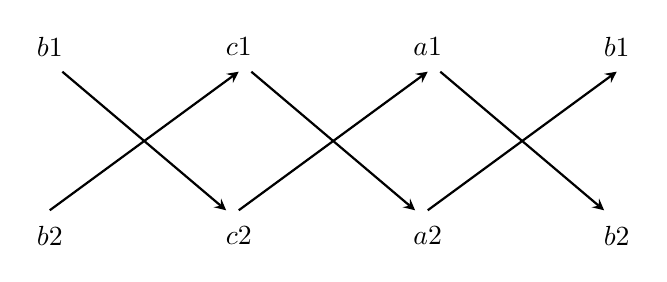
\begin{tikzpicture}[scale=1.6]%
   \draw (0,0) node {$b2$};
   \draw (1.5,0) node {$c2$};
   \draw (3,0) node {$a2$};
   \draw (4.5,0) node {$b2$};
   \draw (0,1.5) node {$b1$};
   \draw (1.5,1.5) node {$c1$};
   \draw (3,1.5) node {$a1$};
   \draw (4.5,1.5) node {$b1$};
   \draw[->, >=stealth, thick] (0, 0.2) -- (1.5, 1.3);
   \draw[->, >=stealth, thick] (1.5, 0.2) -- (3, 1.3);
   \draw[->, >=stealth, thick] (3, 0.2) -- (4.5, 1.3);
   \draw[->, >=stealth, thick] (0.1, 1.3) -- (1.4, 0.2);
   \draw[->, >=stealth, thick] (1.6, 1.3) -- (2.9, 0.2);
   \draw[->, >=stealth, thick] (3.1, 1.3) -- (4.4, 0.2);
\end{tikzpicture}%
\end{document}
